%=================================================================

\section{Introduction}\label{sec-intro}

\subsection{Problem Statement}
\

The data contains the location and circumstances of every field goal 
attempted by Kobe Bryant took during his 20-year career. The task is to predict 
whether the basket went in (shot_made_flag).




\subsection{Data List}
\

The action_type,shot_made_flag,  
shot_type and shot_zone_area are part of the attributes of each sample,
the fllowings are the meaning of some attributes.

		\begin{table}[htbp]
	\centering
	\begin{tabular}{cc}
		\toprule  %????????
		Attribute& Note\\
		\hline
		action_type & Jumpshot,Layup,Dunk,Tipshot,Hookshot,Bankshot\\
		loc_x ,loc_y & shots point\\
		shot_made_flag & 1=Yes,0=No\\
		shot_type & 2PT Field Goal,2PT Field Goal\\
		shot_zone_area & shots area by area\\
		shot_zone_basic & shots area by  NBA rules\\
		shot_zone_range & shots area by radius\\
		
		\bottomrule %????????
	\end{tabular}
	\bigskip
	\caption{Data Information}
\end{table}
\label{table1}



\subsection{Problem Analysis}

\subsubsection{Train Data and Test Data}
\
There are 30697 lines of data in the training set.I will split the dataset as training sets and testing sets.
They have removed 5000 of the shot_made_flags (represented as missing values in the csv file). 
These are the test set shots for which we need submit a prediction. We are provided
a sample submission file with the correct shot_ids needed for a valid prediction.


\subsubsection{Problem Possible Solutions}
\
After analyse the dataset by some simple visualizations.
In the process of date preparation,I will engineer the feature to improve the model accuracy,
then,create some dummy variables.
There are many machine learning moodel
can solve the two classification problem,
such as The RandomForestClassifier,
KNeighbors Classifier and Logistic Regression.
Finaly,make a final prediction,fit the model with whole data





\section{Exploratory Data Analysis} \label{sec-data_exploration}

\subsection{Data Information}
\

The following  ~\cref{tbl:data information}
is the statistical result of the columns.
From this table,we can discover that some of columns have a similar meaning 
or may not contribute much to the model.
so we may need remove and convert them. 

\begin{table}[htbp]  \centering
	\caption{Data Information}
	\label{tbl:data information}		
	\begin{tabular}{ccccccc}
		\hline
		% after \\: \hline or \cline{col1-col2} \cline{col3-col4} ...
		& lat & loc\_x & loc\_y & lon & minutes\_remaining & seconds\_remaining & shot\_distance\\
		\hline
		count & 30697.000000 & 30697.000000 & 30697.000000 & 30697.000000 & 30697.000000 & 30697.000000 & 30697.000000 \\
		mean & 33.953192 & 7.110499	& 91.107535 & -118.262690 & 4.885624 & 28.365085 & 13.437437 \\
		std & 0.087791	& 110.124578 & 87.791361 & 0.110125	& 3.449897 & 17.478949 & 9.374189 \\
		min & 33.253300	& -250.000000 & -44.000000 & -118.519800 & 0.000000	& 0.000000 & 0.000000 \\
		25\% & 33.884300 & -68.000000 & 4.000000 & -118.337800 & 2.000000 & 13.000000 & 5.000000 \\
		50\% & 33.970300 & 0.000000	& 74.000000	& -118.269800	& 5.000000	& 28.000000	& 15.000000\\
		75\% & 34.040300 & 95.000000 & 160.000000 & -118.174800 & 8.000000 & 43.000000 & 21.000000\\
		max & 34.088300 & 248.000000 & 791.000000 & -118.021800 & 11.000000 & 59.000000 & 79.000000\\
		\hline 
		%\bottomrule
	\end{tabular}
\end{table}


\subsection{Data Visualization}
\

Use EDA to plot the distribution of the data,
can observate the data intuitively and
find the relation between the attribute values. 
For example histogram can visually observe 
the distribution of numerical variables, 
scatterplot can show their distribution trends 
and whether exists outliers.
For classification problems, 
the data with the same label is drawn in same color, 
which is very helpful for 
the construction of the Feature.


\subsubsection{ Histogram}
\

The figure ~\Cref{fig:c} 
shows the hit distribution of Kobe's shots  
the figure ~\Cref{fig:d} 
is the visualization of two kinds of shots(two-point shot and three-point shot).
It can be seen that the number of shots and hit rate of the 2PT ball are extremly high. 
While the percentage of 3PT shots is relatively low.
the figure ~\Cref{fig:f} 
shows the shot accuracy of various action type.
It can be seen that dunk is the highest hit rate, followed by bank shot is about 80\%,
 while jump shot and Tip shot are relatively difficult.



\begin{figure}[htbp]
	\centering
	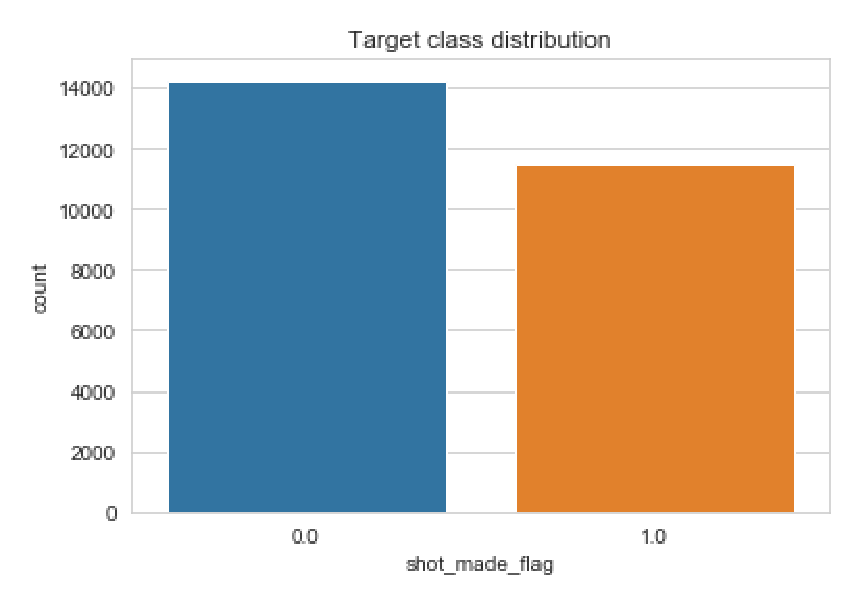
\includegraphics[scale=0.8]{c.eps}        %?a??¨º??¨²LaTeX???t?D?D¦Ì??¨¤???¡¤??
	\caption{target class distribution}
	\label{fig3}
\end{figure}
\begin{figure}[htbp]
	\centering
	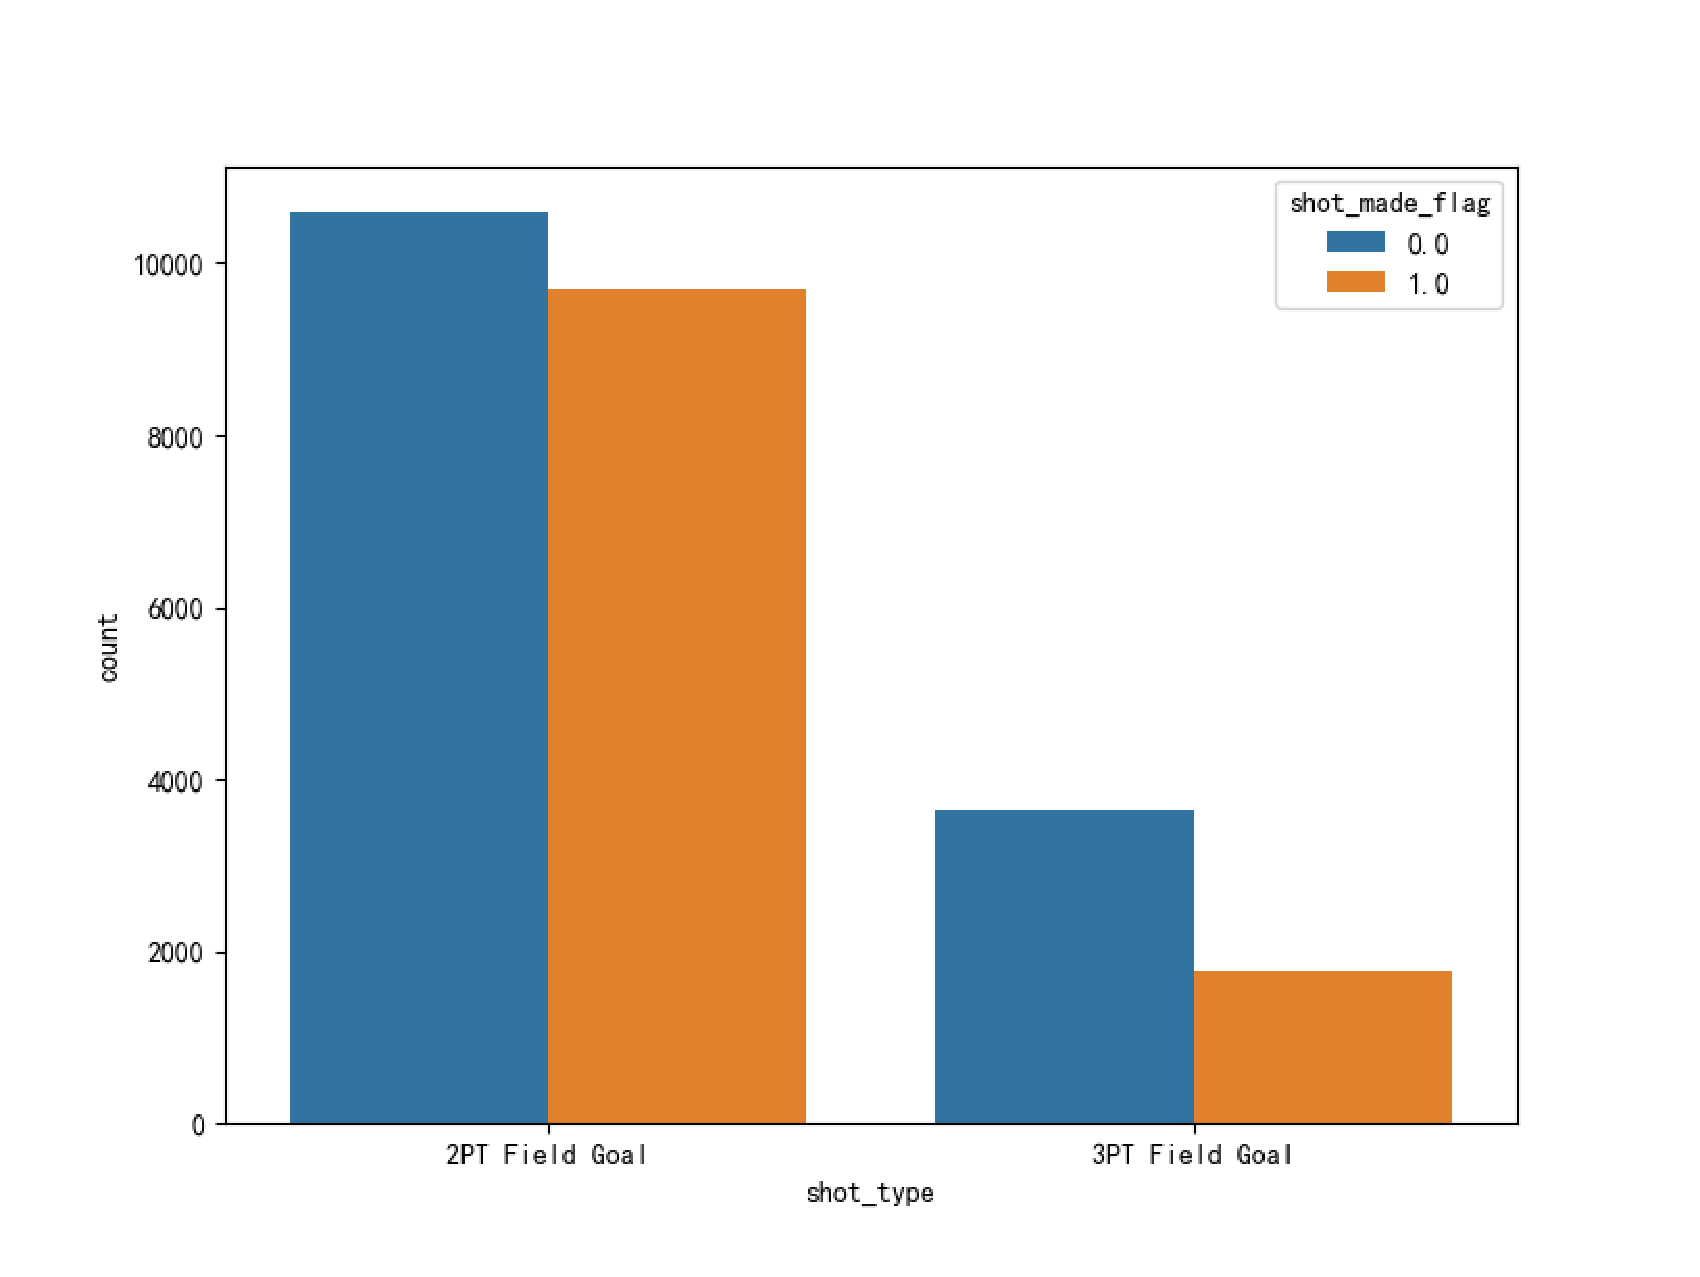
\includegraphics[scale=0.3]{d.eps
	}        %?a??¨º??¨²LaTeX???t?D?D¦Ì??¨¤???¡¤??
	\caption{The hit distribution histogram of two shot types}
	\label{fig4}
\end{figure}

\begin{figure}[htbp]
	\centering
	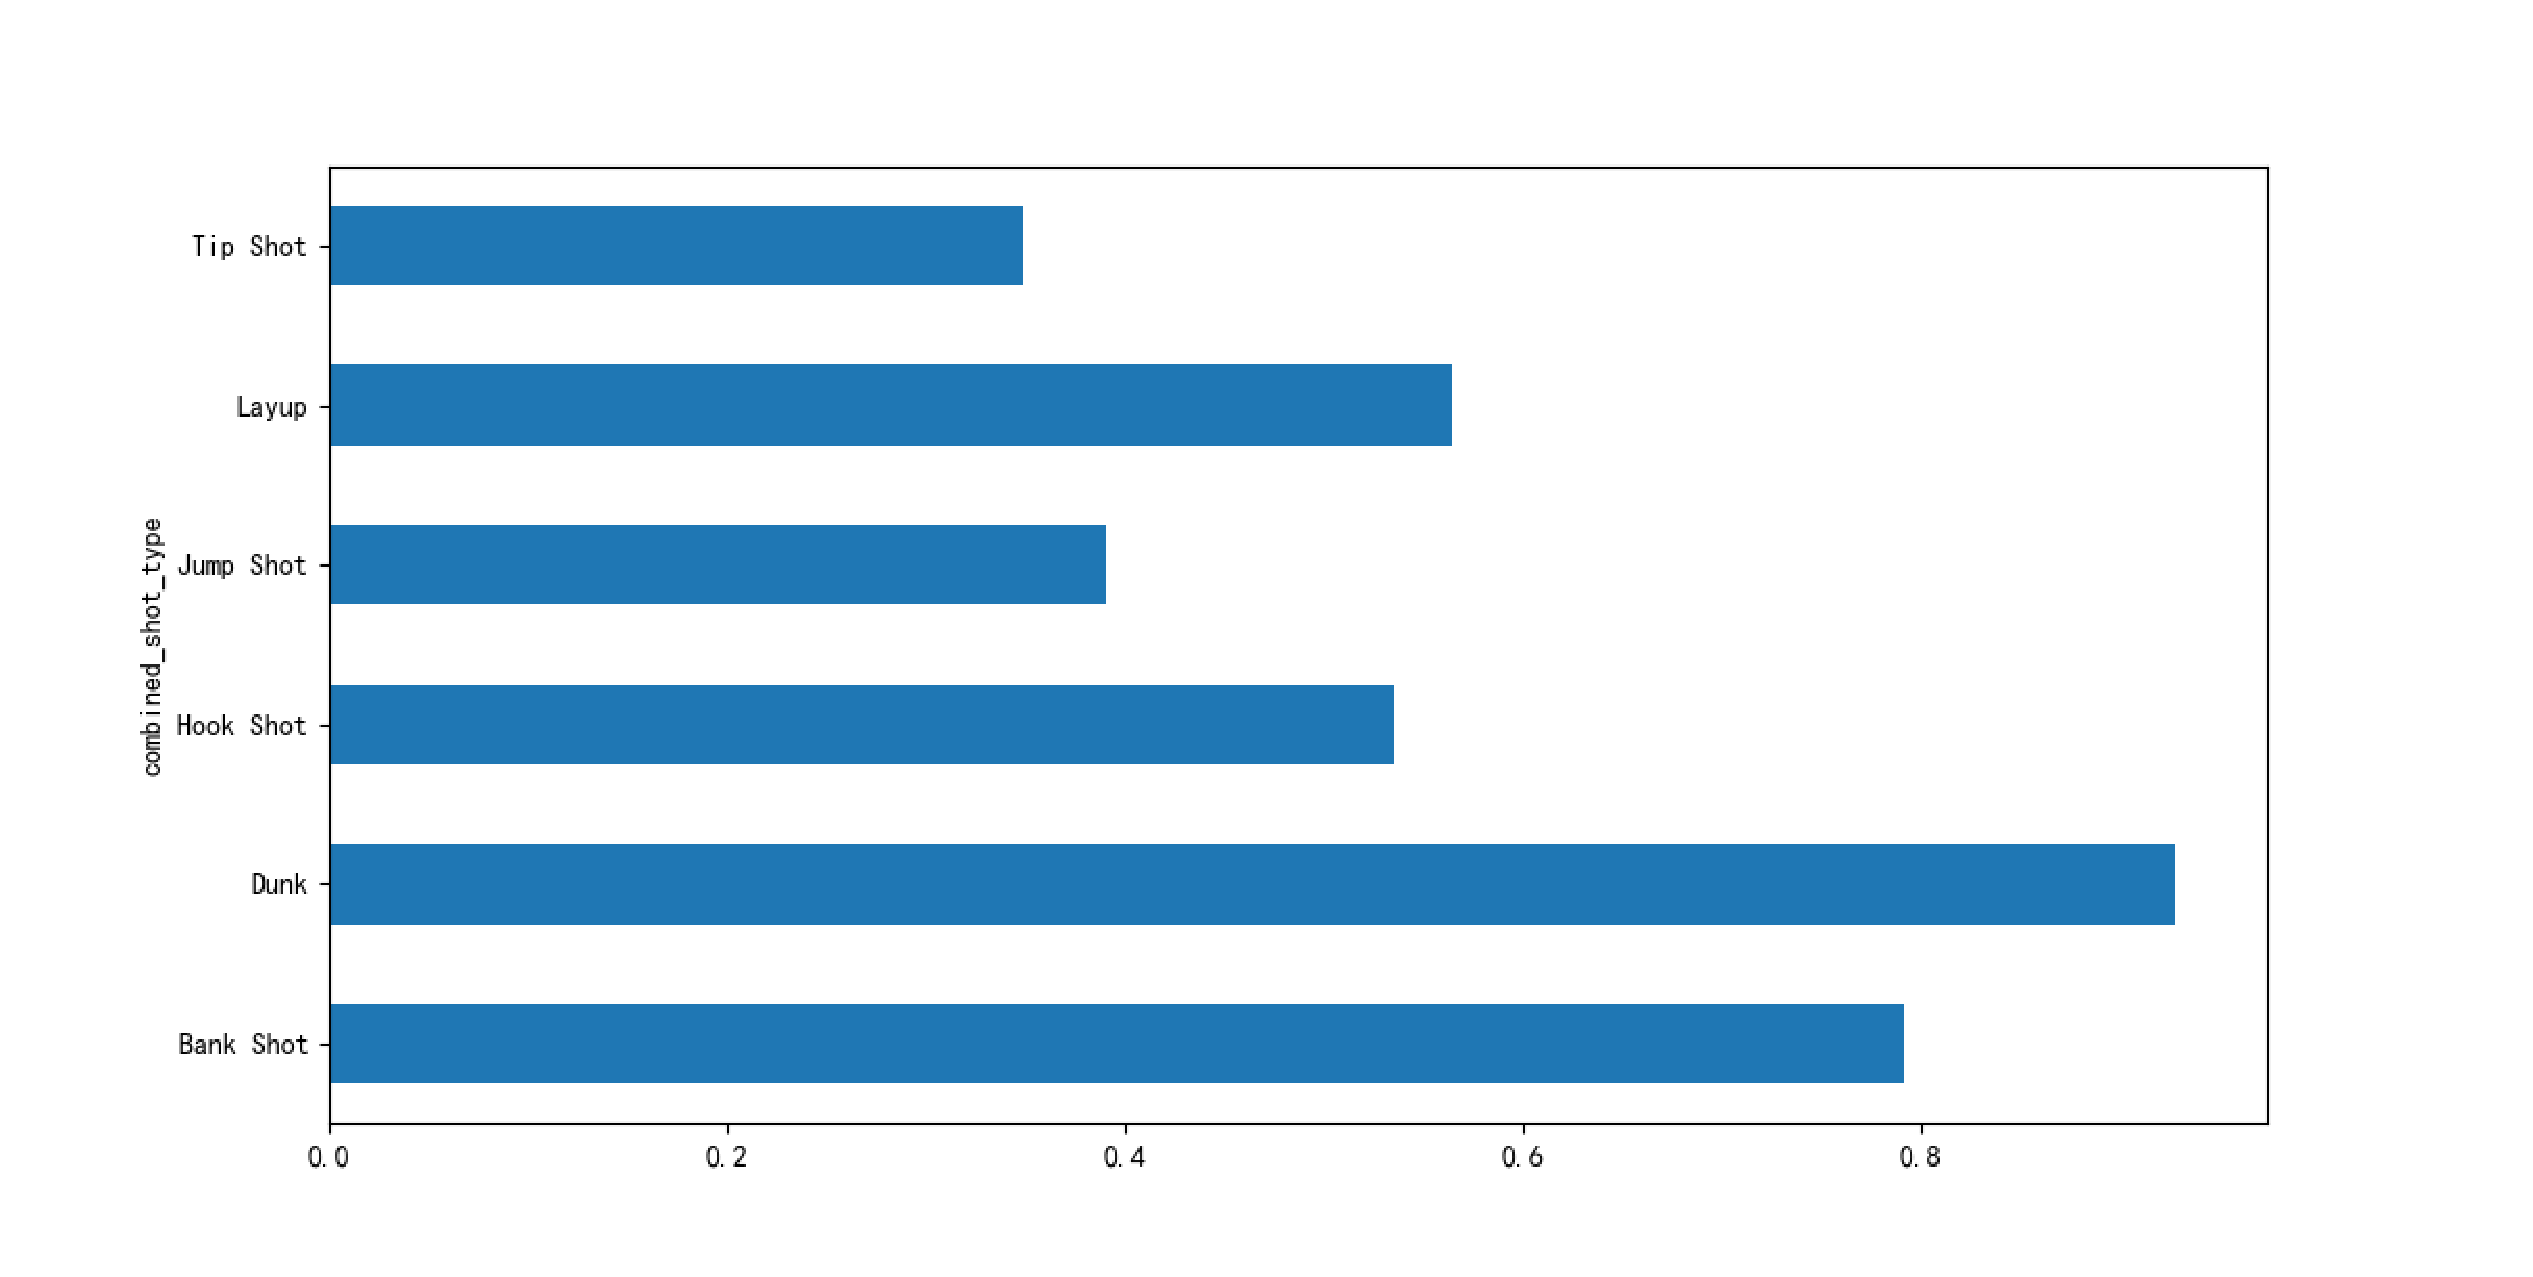
\includegraphics[scale=0.4]{f.eps
	}        %Õâ¸öÊÇÔÚLaTeXÎļþ¼ÐÖеÄÏà¶Ô·¾¶
	\caption{the shot accuracy of various action type}
	\label{fig6}
\end{figure}

\subsubsection{Scatter plot}
\
 
Using the scatter plot we can combine multiple 
categorical value series on to the same chart distinguishing them using color or 
variation in symbol.
Lets get some understanding about the different zones and the shots made from zones.

\begin{figure}[htbp]
	\centering
	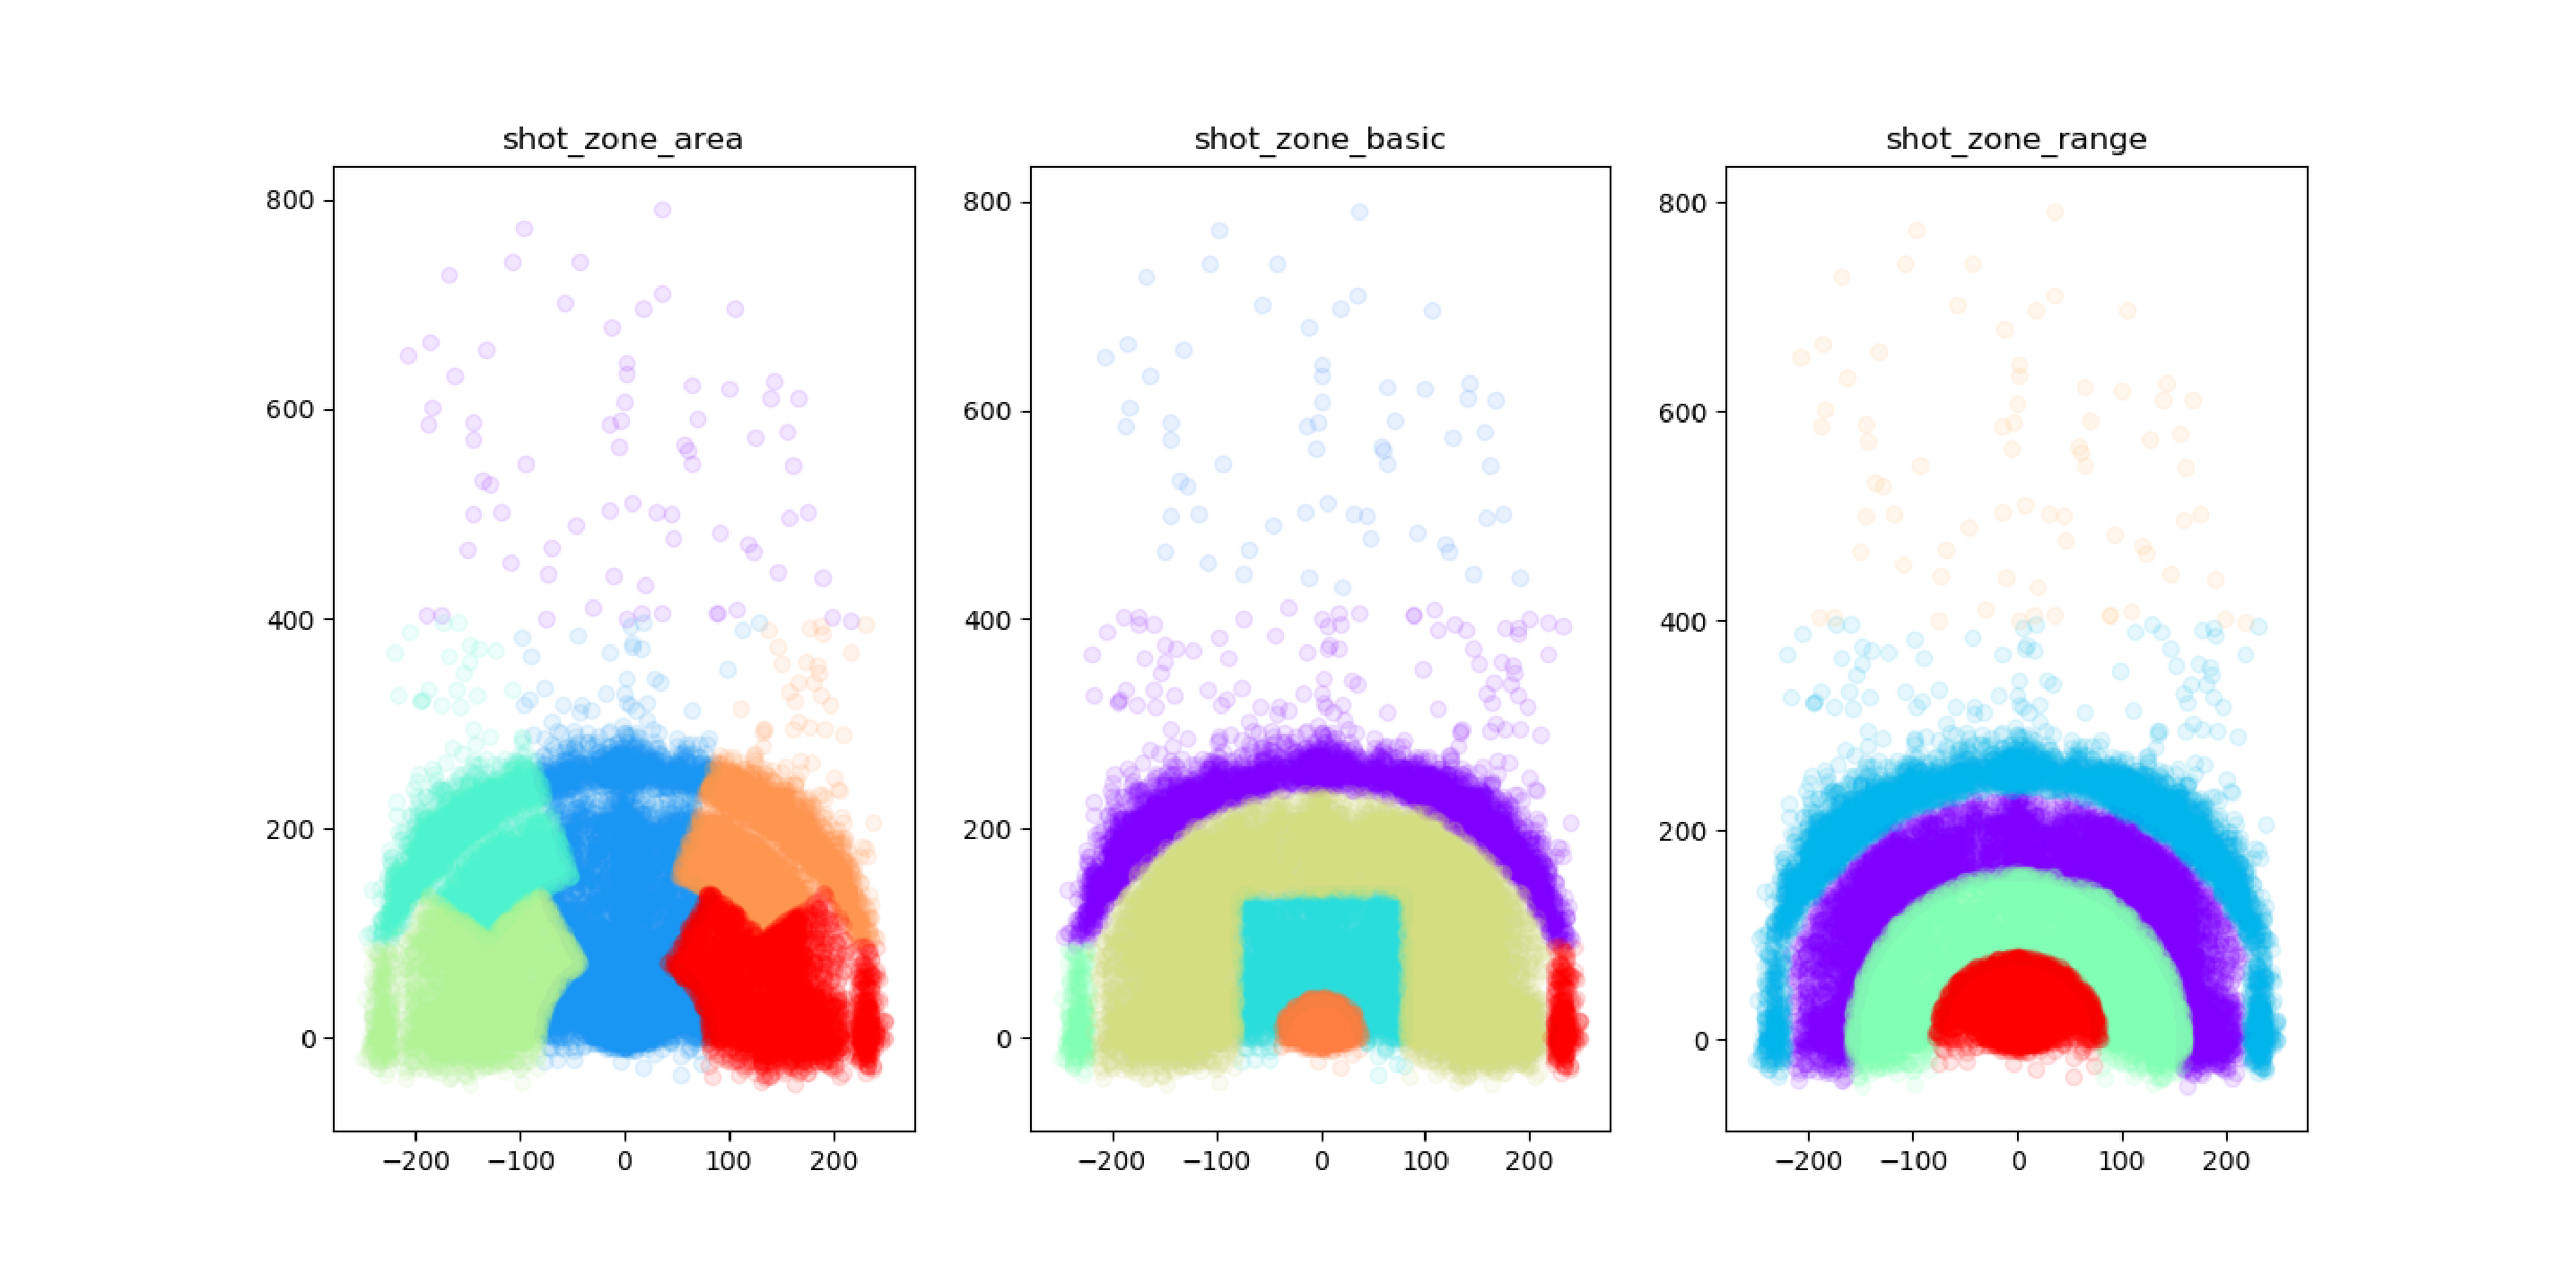
\includegraphics[scale=0.3]{h.eps
	}        %Õâ¸öÊÇÔÚLaTeXÎļþ¼ÐÖеÄÏà¶Ô·¾¶
	\caption{Division of shooting area}
	\label{fig8}
\end{figure}

\subsubsection{Line Chart}
\

The line chart can not only show the quantity, but also clearly see the increase and decrease of data.
Lets now see the Kobe's shots positioning with the time and distance.

\begin{figure}[htbp]
	\centering
	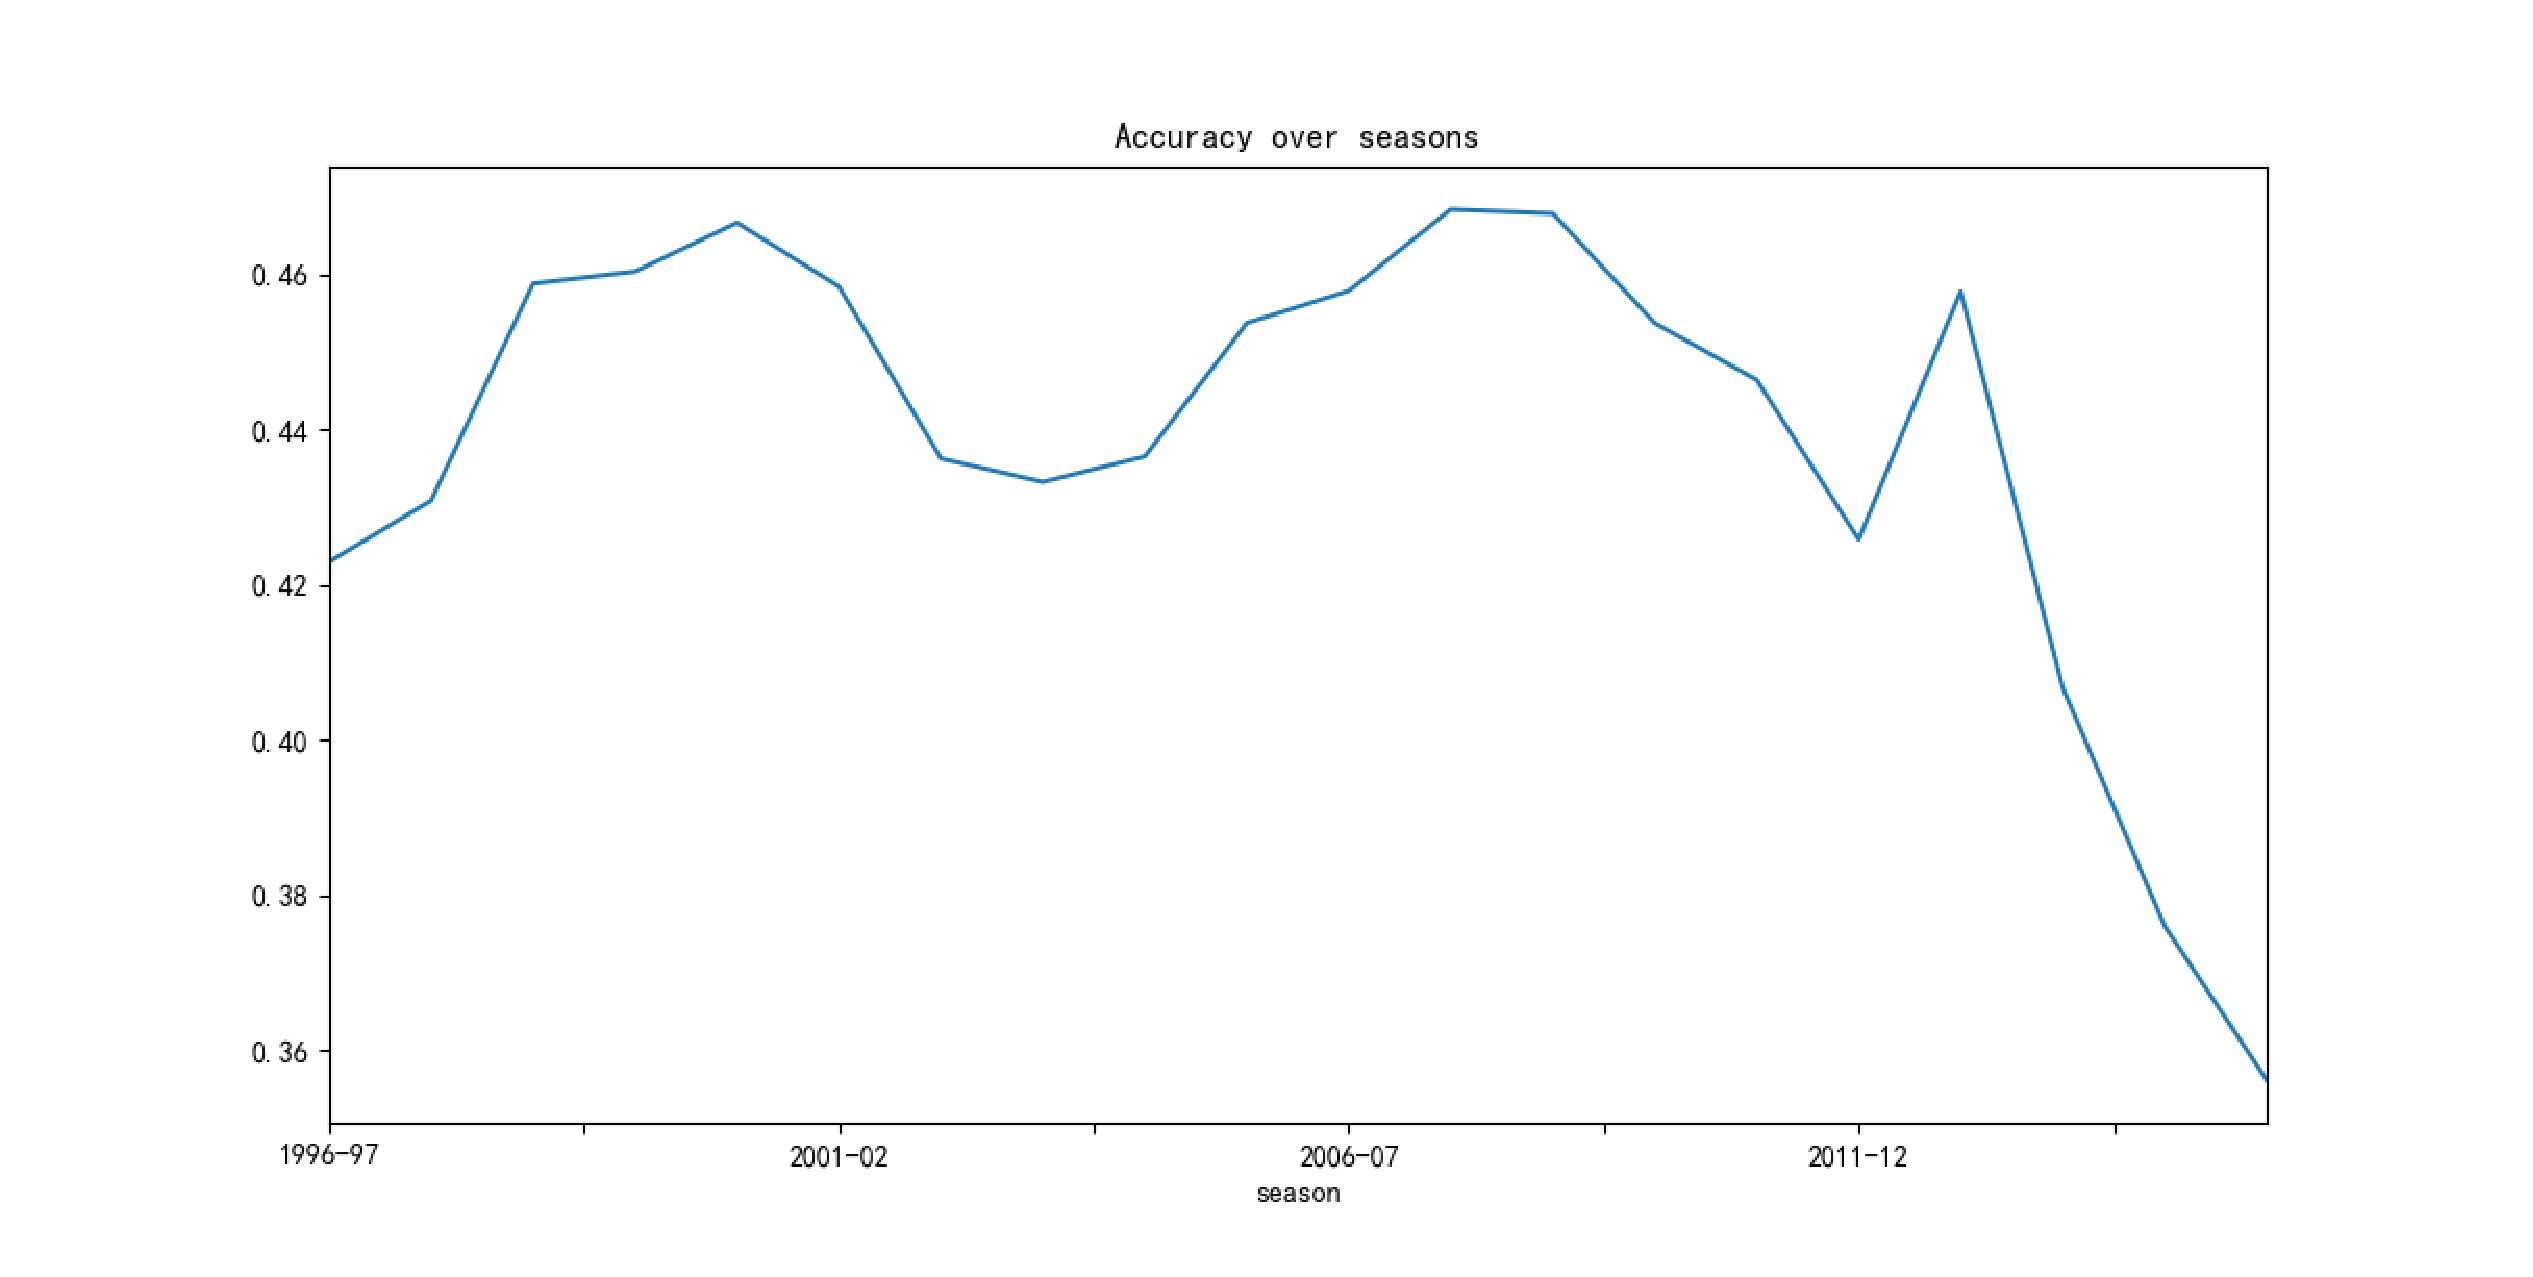
\includegraphics[scale=0.4]{m.eps
	}        %Õâ¸öÊÇÔÚLaTeXÎļþ¼ÐÖеÄÏà¶Ô·¾¶
	\caption{shot accuracy of each seasons}
	\label{fig12}
\end{figure}

\begin{figure}[htbp]
	\centering
	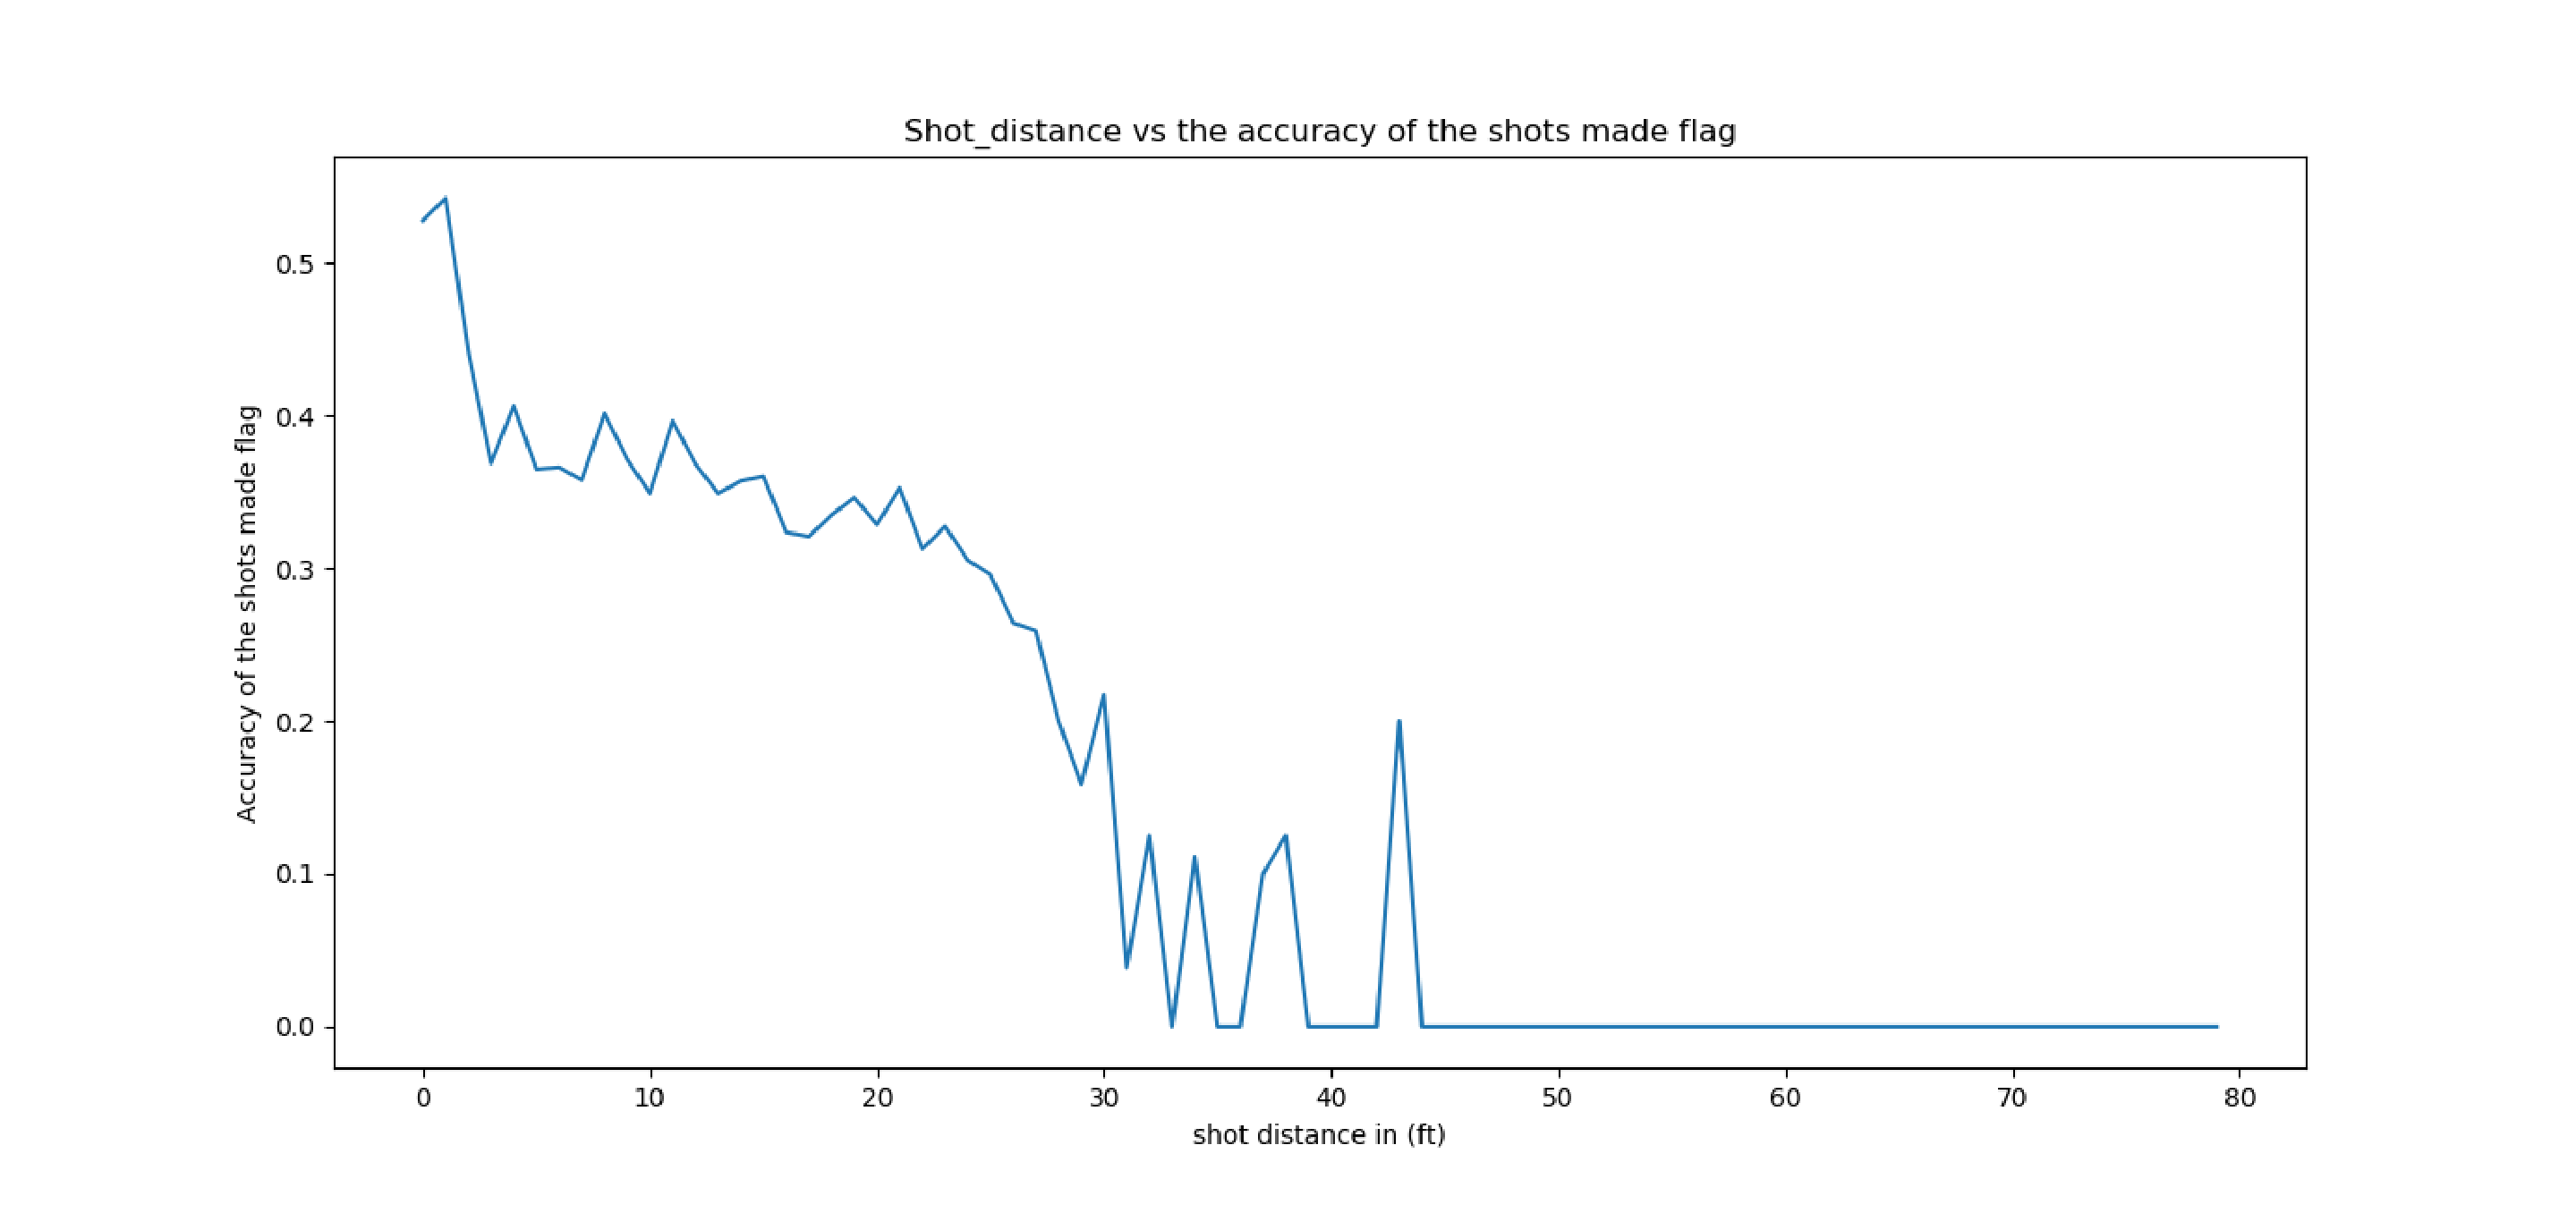
\includegraphics[scale=0.3]{s.eps
	}        %Õâ¸öÊÇÔÚLaTeXÎļþ¼ÐÖеÄÏà¶Ô·¾¶
	\caption{Shot_distance vs the accuracy of the shots made flag}
	\label{fig8}
\end{figure}

\subsection{Data Preparation}

\subsubsection{Data Cleaning}
\

As it can be seen from 
the picture that, (loc_x ,loc_y) and (lat , lon) represent the same.
So, drop one of those.
Meanwhile,some attributes have no attribution for our model,
Therefore some columns might be dropped.
similarly,there is no real use of the columns team_id, team_name, game_event_id, game_id.
So, removing them is a good option.The opponent and the matchup also represents the same thing, 
so remove the matchup column.The game_date and shot_id also has no use.
Since, we have equal attacks from both sides we can remove the shot_zone_ares as it
 doesnt contribute much to the model, we can also remove the shot_zone_basic for the same reason.


\begin{figure}[htbp]
	\centering
	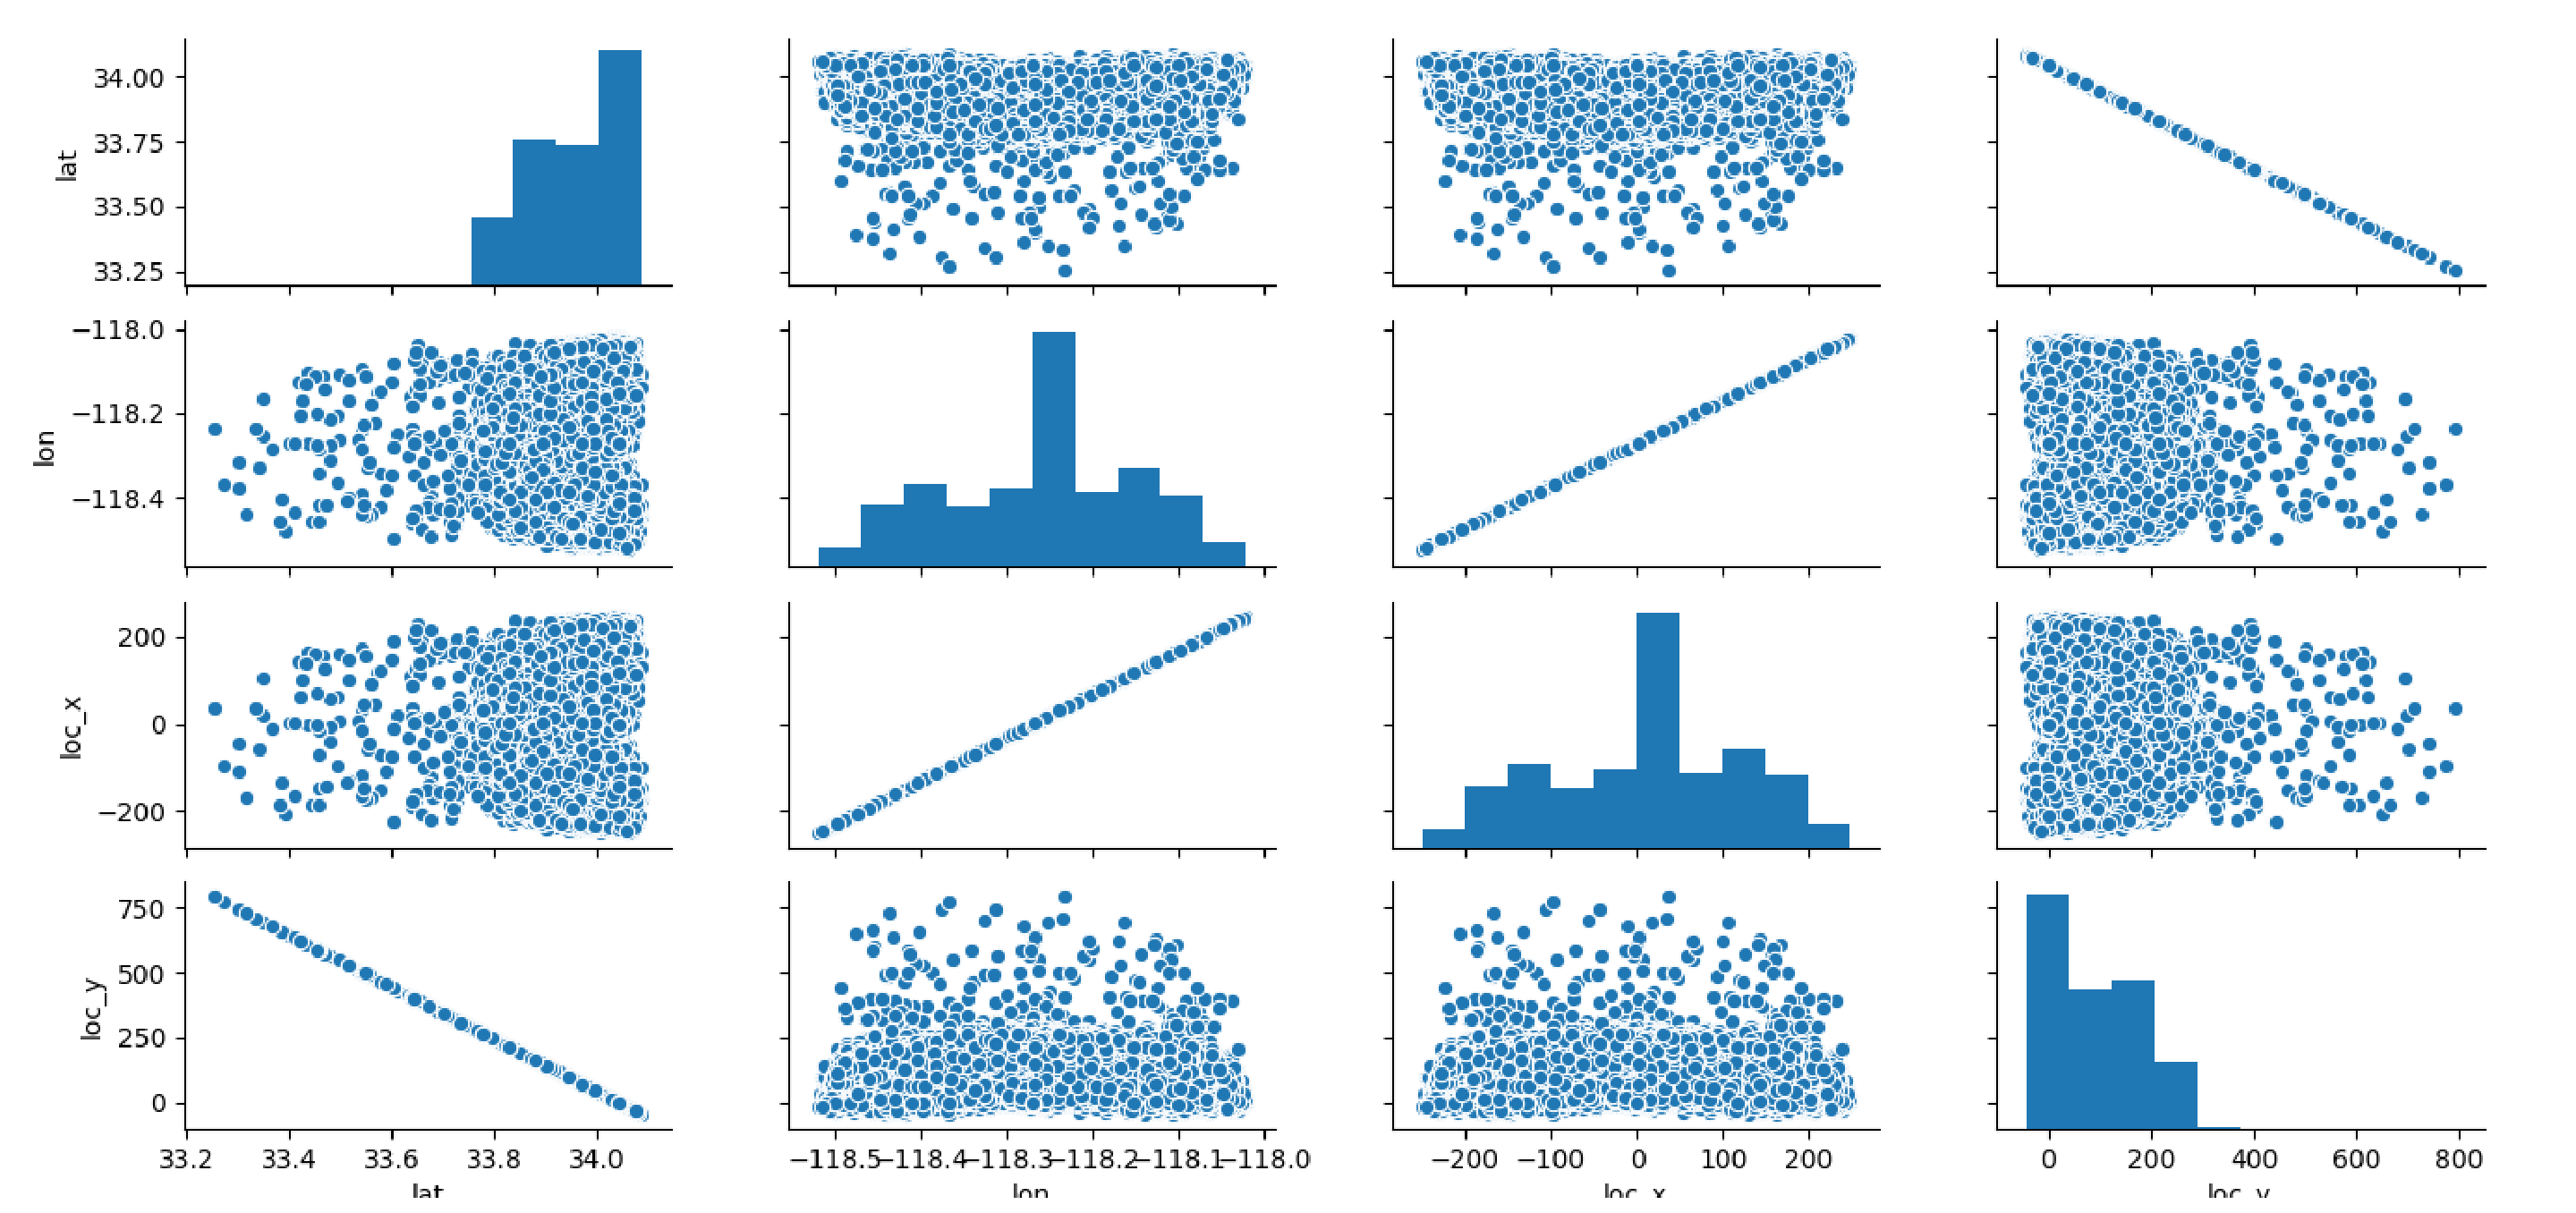
\includegraphics[scale=0.3]{t.eps
	}        %Õâ¸öÊÇÔÚLaTeXÎļþ¼ÐÖеÄÏà¶Ô·¾¶
	\label{fig8}
\end{figure}


\subsubsection{Data Transformation}
\
After deleted all the useless columns,we need to merge some features,and create the dummy variables.
First,Let's convert the minutes and seconds to single column.
\begin{description}
	\item[total\_seconds] row[seconds\_remaining]*row[seconds\_remaining] 
\end{description}
After that,we can remove the minutes and the seconds columns.
Categorical variables such as action_type,combined_shot_type,season,shot_type,shot_zone_range 
and opponent,we can create the dummy variables for further analysis.
\begin{figure}[htbp]
	\centering
	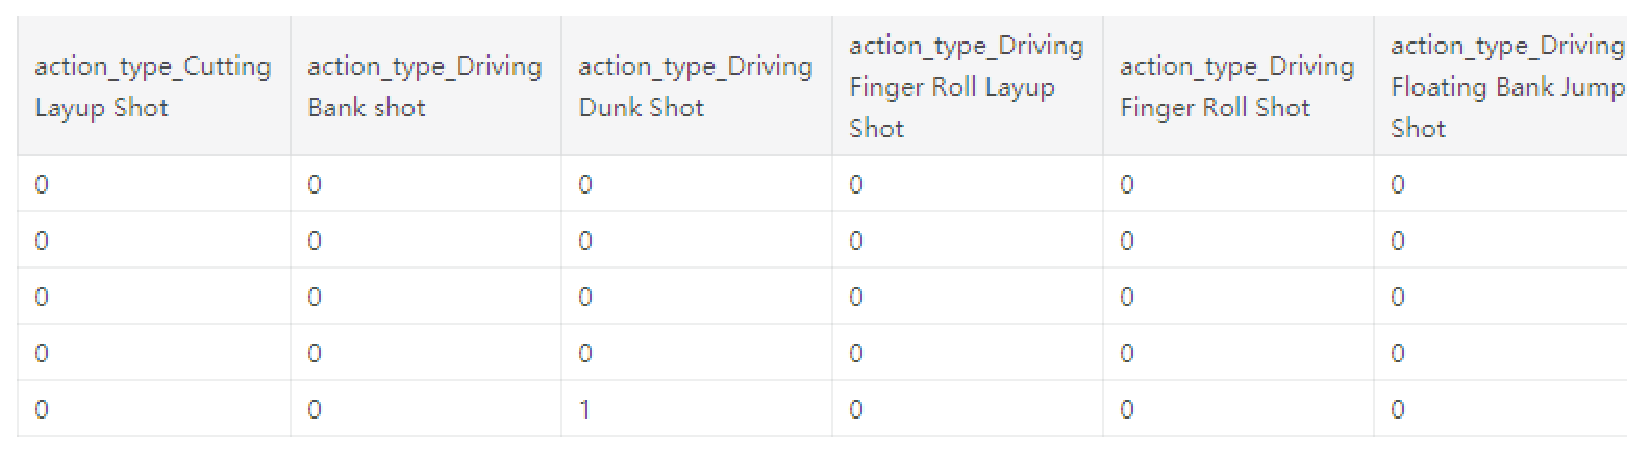
\includegraphics[scale=0.3]{u.eps
	}        %Õâ¸öÊÇÔÚLaTeXÎļþ¼ÐÖеÄÏà¶Ô·¾¶
	\label{fig8}
\end{figure}

\section{Methods}

There are many machine learning algorithms 
for classification problem. 
Choose the following algorithms
as the base models of ensemble model,show the most important parameters.

\begin{itemize}
	\item RandomForest 
	%\item Bagging
	%\item GradientBoosting
	\item LogisticRegression
	\item SVC
	\item KNeighbors 
	\item XGBoost
	\item Netual Network
\end{itemize}
\subsection{Base Models}
\

The base models have many parameters,
select the some parameters that 
have a larger impact on 
the forecast results,
the use Grid Search to find 
the optimal paratemers set.	
The following is training result. 
\subsubsection{RandomForest}
\

Random forest is a classifier with 
multiple decision trees, and
the output is determined by 
the mode of the individual tree output.


\begin{description}
	\item[n_estimators] the number of decision trees
	\item[criteriom] criterion of choosing 
	the most appropriate node
	\item[max_depth] The maximum depth of the tree, 
	the default is None 
	\item[max_features] The feature that is divided 
	when selecting the optimal attribute 
	cannot exceed this value.
\end{description}




\subsubsection{LogisticRegression}
\

Logistic regression is the algorithm that 
processing a large amount of 
observation data to 
obtain mathematical expressions 
that are in line with 
the internal laws of things
	
	
\begin{description}
	\item[Penalty] Regular function
	\item[C] Regular coefficient
\end{description}
	
%J=sum(logloss(f(xi), yi)) + C* penalty


%\frac{\partial f}{\partial x} = 2\,\sqrt{a}\,x
\subsubsection{SVC}
\

The basic principle of the SVM algorithm is 
to find a hyper plane that can 
distinguish between two types, 
so that the margin is the largest.


\begin{description}
	\item[kernel] kernel function
	\item[C] penalty factor for error terms
	\item[degree] order of polynomial kernel function
\end{description}
	
\subsubsection{KNeighbors}
\

The meaning of the knn algorithm is that 
enter new data without tags, 
compare each feature of the new data with 
each feature in the training set, 
and select the classification tag with 
the most similar feature (nearest neighbor: k)


\begin{description}
	\item[n_neighbors] number of neighbors to use 
	by default for kneighbors queries
	\item[leaf_size] leaf size passed to BallTree or KDTree
	\item[p] power parameter for choosing 
	the distance calculation formula
	\item[weights] used in prediction
	\item[algorithm] compute the nearest neighbors
	\end{description}
	
\subsubsection{XGBoost}
\
 
XGBoost is to establish K regression trees 
so that the predicted value of 
the tree group is as close as possible to 
the true value (accuracy) and 
has the greatest generalization ability. 
From a mathematical point of view, 
this is a functional optimization, multi-target.

\begin{description}
	\item[learning_rate]  control the speed of each update
	\item[n_estimators] number of iterations
	\item[max_depth] the depth of tree
	\item[gamma] penalty factor%惩罚系数
	\item[subsample] the proportion of data used in 
		all training sets when training each tree
	\item[colsample_bytree] the proportion of features used 
		in all trees when training each tree
	\end{description}

\subsubsection{Netual Network}
\

Netual network is widely used in various fields.
It generally consists of 
an Input Layer, a Hidden Layer, and an Output Layer. 
Each layer is composed of Units. 
	
	
\begin{description}
	\item[hidden_layer_sizes] The i-th element represents 
		the number of neurons in the i-th hidden layer
	\item[activation] activation function
	\item[solver] weight optimization solver
	\item[learning_rate] weight update speed
\end{description}


\subsection{Ensemble Model}
\

There are many machine learning algorithms, 
use the above machine learning algorithms 
as Ensemble Model’s base models. 
Through Grid Search and
ten-fold cross-validation
to find the optimal parameters.

\section{Experiment and Analysis}

In the Data Exploration, 
I has created some new feaures.
The following experiment is divided into two parts,
one is to use the original train data, 
the other is to use new features as train data.
Grid Search make it easier to 
determine a set of optimal parameters
for these model I adpot.
Because the train data is relatively small, 
a ten-fold cross-validation is used. 
Then I can test the trained models 
using test data and 
analyze the experimental results.
And use the trained models as 
the base models of ensemble model,
then do experiment. 
%\WBJianginMarker

\subsection{Base Models Training Result}
\subsubsection{Original Train Data}
\

The following are the best parameters and 
the Best Score in training of 
the base models 
in original train data. 

\begin{itemize}
	\item Best Parameters of Models
	\begin{description}
		\item[RandomForest] 'criterion': 'entropy', 'max_depth': 5, 
		'max_features': None, 'n_estimators': 100
		\item[LogisticRegression] 'C': 1, 'penalty': 'l1'
		\item[SVC] 'C': 10, 'degree': 3, 'kernel': 'linear'
		\item[KNeighbors] 'algorithm': 'auto', 'leaf_size': 10, 
		'n_neighbors': 20, 'p': 5, 'weights': 'uniform'
		\item[XGBoost] 'learning_rate':0.08,'n_estimators':50,
		'max_depth':5,
		
		'gamma':0,'subsample':0.9,'colsample_bytree':0.5
		\item[Netual Network] 'activation': 'relu', 'hidden_layer_sizes': 9, 
		'learning_rate': 'adaptive', 'solver': 'adam'
	\end{description}
	
	\item Best Score in Ten-Fold Cross-Validation
	
	From the  ~\Cref{tbl:best_score_base_models_old},
	it shows that the accuracy of 
	each model is not much different,
	except XGBoost.
	
	\begin{table}[h]  \centering
		\caption{Best Score of the Base Models}
		\label{tbl:best_score_base_models_old}
		\begin{tabular}{ccccccc}
			%\bottomrule
			\toprule
			& RF  & LR & SVC & KNN & XGBoost & Netual Network\\
			\midrule
			Best Score & 0.7224  & 0.7547 & 0.7493 & 0.7251 & 0.9314 & 0.7466\\
			\bottomrule
		\end{tabular}
	\end{table}
\end{itemize}

\subsubsection{New Train Data}
\

The following are the base models 
with the best parameters 
provided by Grid Search.

\begin{itemize}
	\item Best Parameters of Models
	\begin{description}
		\item[RandomForest] 'criterion': 'entropy', 'max_depth': 5, 
		'max_features': 'auto', 'n_estimators': 100 
		\item[LogisticRegression] 'C': 10, 'penalty': 'l2'
		\item[SVC] 'C': 5, 'degree': 3, 'kernel': 'rbf'
		\item[KNeighbors] 'algorithm': 'auto', 'leaf_size': 10, 
		'n_neighbors': 10, 'p': 2, 'weights': 'uniform' 
		\item[XGBoost] 'learning_rate':0.07,'n_estimators':50,
		'max_depth':6,
		
		'gamma':0,'subsample':0.9,'colsample_bytree':0.5
		\item[Netual Network] 'activation': 'identity', 
		'hidden_layer_sizes': 8, 'learning_rate': 'adaptive', 'solver': 'adam'
	\end{description}
	
	\item Best Score in Ten-Fold Cross-Validation
	
	Compare with the  ~\Cref{tbl:best_score_base_models_old}
	above,
	you can find that the accuracy of the models increases,
	although it's not obvious.
	
	\begin{table}[h]  \centering
		\caption{Best Score of the Base Models}
		\label{tbl:best_score_base_models_new}
		\begin{tabular}{ccccccc}
			\toprule
			% after \\: \hline or \cline{col1-col2} \cline{col3-col4} ...
			& RF & LR & SVC & KNeighbors & XGBoost & Netual Network\\
			\midrule
			Best Score & 0.7224 & 0.7547 & 0.7493 & 0.7251 & 0.9326 & 0.7466\\
			\bottomrule
		\end{tabular}
	\end{table}
\end{itemize}

\subsection{Forecast Result of Base Models}
\

From the table below
shows the result of base models
on test data.
Some models have improved accuracy, 
but some models have reduced accuracy.

\begin{table}[h]\centering
	\caption{Forecast Result of Base Models}
	\begin{tabular}{ccccccccc}
		\toprule
		& Acc_old & Acc_new & Prec_old & Prec_new & Rec_old & Rec_new & F1_old & F1_new\\
		\midrule
		RF & 0.81 &      0.83 & 0.84 & 0.84 & 0.81 & 0.83 & 0.82 & 0.83\\
		LR & 0.76 &      0.75 & 0.76 & 0.75 & 0.76 & 0.75 & 0.76 & 0.75\\
		SVC & 0.75 &     0.69 & 0.77 & 0.71 & 0.75 & 0.69 & 0.75 & 0.70\\
		KNN & 0.73 &     0.71 & 0.77 & 0.73 & 0.73 & 0.71 & 0.74 & 0.71\\
		XGBoost & 0.92 & 0.95 & 0.92 & 0.95 & 0.92 & 0.95 & 0.92 & 0.95\\
		NN & 0.73 &      0.68 & 0.75 & 0.71 & 0.73 & 0.68 & 0.74 & 0.69\\
		mean $\pm$ var & .78$\pm$.005 & .77$\pm$.009 &
		.80$\pm$.004 & .78$\pm$.008 &
		.78$\pm$.005 & .77$\pm$.009 &
		.79$\pm$.004 & .77$\pm$.009\\	
		\bottomrule
	\end{tabular}
\end{table}

\subsection{Forecast Result of Ensemble Model }
\

Ensemble model means using 
more than 1 model to finish the prediction.
Here just averaging the prediction results 
by using voting. 

\subsubsection{Original Train Data}
\

The table below is the metrics classification report 
of ensemble model in original train data.

\begin{table}[h]  \centering
	\caption{Metrics Classification Report of Ensemble Model}
	\label{tbl:metrics_classification_ensemble_old}
	\begin{tabular}{ccccc}
		\hline
		& precision  &  recall & f1-score &  support\\
		\hline
		Ghost   &    0.80   &   0.83  & 0.82 & 24\\
		Ghoul  &  0.88  &  0.79  &   0.84   &   29\\
		Goblin  &   0.67  &  0.73 &  0.70  &   22\\
		\hline
		micro avg  &  0.79  &  0.79  & 0.79    &  75\\
		macro avg  &  0.78  & 0.78  &  0.78  &  75\\
		weighted avg  &   0.79  &  0.79 &  0.79  &  75\\
		\hline 
		%\bottomrule
	\end{tabular}
\end{table}

\subsubsection{New Train Data}
\

The table below is the metrics classification report 
of ensemble model in new train data.
\begin{table}[h]  \centering
	\caption{Metrics Classification Report of Ensemble Model}
	\label{tbl:metrics_classification_ensemble_new}
	\begin{tabular}{ccccc}
		\hline
		&precision & recall & f1-score & support\\
		\hline
		Ghost  &  0.84  &  0.88  & 0.86 &  24\\
		Ghoul  &  0.93  & 0.97 &  0.95 &   29\\
		Goblin  &  0.80 &  0.73  & 0.76  &  22\\
		\hline
		micro avg & 0.87  & 0.87  & 0.87  & 75\\
		macro avg &  0.86  &  0.86 & 0.86 &   75\\
		weighted avg  &  0.86 & 0.87  &  0.86  &  75\\
		\hline 
		%\bottomrule
	\end{tabular}
\end{table}	


\section{Conclusion}

\begin{itemize}
	\item Exploratory data analysis is 
	very important for the competition,
	that is an exploratory analysis 
	of the data to 
	provide the necessary conclusions 
	for data processing and modeling. 
	\item The data that we have,
	needed processed in many cases.
	Data preprocessing includes 
	deal with missing data and outliers,
	change categorical variable 
	into one-hot code and so on.
	\item The most important thing is
	feature engineering.
	We can create as more as poosible features,
	then select the most useful features.
	\item Model training is also very important.
	There are many algorithms, 
	in my opinoin, 
	if the time permits,
	we can We can try all the algorithms. 
	\item The last thing is adjustment,
	for example,
	the models have many parameters,
	can use Grid Search to find 
	the optimal paratemers.	
\end{itemize}

%\lstset{language=python}         
%\begin{lstlisting}[frame=single]  % Start your code-block
%rf = RandomForestClassifier(random_state = 0)
%clf = GridSearchCV(rf, param_grid = params, scoring = accuracy_scorer, cv = 10, n_jobs = -1)
%clf.fit(X_train, y_train)
%y_pred = clf.predict(X_test)
%\end{lstlisting}










